%

\subsection{Library \protect\library{file}}
The library \library{file} draws files and uses \library{record}.

\usedslibrary{file}

\subsubsection{Drawing files horizontally}
Horizontal file with records.




\begin{tcblisting}{}
\begin{tikzpicture}
	\dsfilestructure[block size = 4096, kbyte width = 15em,
		structure offsets
	]{
		R$_0$/500,
		R$_1$/1300,
		R$_2$/1800,
		R$_3$/900,
		R$_4$/850
	}
\end{tikzpicture}
\end{tcblisting}


\subsubsection{Drawing files vertically}

Files and records are drawn in vertical mode, one record at a time. All records must be defined with \verb|\dsnewnamedrecord| and multiple record formats can be used. \verb|\dsfilenamedrecord| is used to put each record.

\begin{tcblisting}{}
\dsnewnamedrecord{fixed_length}{
	\dsfieldfixed*{12},
	\dsfieldfixed*{2},
	\dsfieldfixed*{18}
}
\dsnewnamedrecord{variable_length}{
	\dsfieldterminator*,
	\dsfieldprefixed*
}

\begin{tikzpicture}[]
	\usedslibrary{file}

	% environment for a file
	\begin{dsfile}
		\dsfilenamedrecord{fixed_length}{Grace, 22, UK}
		\dsfilenamedrecord{fixed_length}{Roberta, 31, Brazil},
		\dsfilenamedrecord{variable_length}{Karl~Ulrich, Germany},
		\dsfilenamedrecord{fixed_length}{Bethany, 34, USA}
		\dsfilenamedrecord{variable_length}{Sandoval, Chile},
	\end{dsfile}
\end{tikzpicture}
\end{tcblisting}


If all records share the same format, \verb|\dsfilerecords| can be used to set records in an easier way. Both \verb|\dsfilerecords| and \verb|\dsfilenamedrecord| can be intermixed.

\begin{tcblisting}{}
\dsnewnamedrecord{record}{
	\dsfieldfixed*{12},
	\dsfieldspace\dsfieldfixed*{2},
	\dsfieldspace\dsfieldfixed*{18}
}

\begin{tikzpicture}[]
	\begin{dsfile}[show frame, show offsets]
		\dsfilerecords{record}{
			{Grace, 22, UK},
			{Roberta, 31, Brazil},
			{Ulrich, 12, Germany},
			{Bethany, 34, USA}
		}
	\end{dsfile}
\end{tikzpicture}
\end{tcblisting}

Blocks

\begin{tcblisting}{}
\dsnewnamedrecord{record}{
	\dsfieldfixed*{12},
	\dsfieldspace\dsfieldfixed*{2},
	\dsfieldspace\dsfieldfixed*{18}
}

\begin{tikzpicture}
	\begin{dsfile}[records = 5, show offsets]
		\begin{dsblock}{record}
			\dsfilerecords{record}{
				{Grace, 22, UK},
				{Roberta, 31, Brazil}
			}
		\end{dsblock}

		\begin{dsblock}{record}
			\dsfilerecords{record}{
				{Karl, 18, Germany},
				{Ulrich, 12, Germany},
				{Bethany, 34, USA}
			}
		\end{dsblock}
	\end{dsfile}
\end{tikzpicture}
\end{tcblisting}


\subsubsection{References}

\begin{tcblisting}{}
\dsnewnamedrecord{record}{
	\dsfieldfixed*{15},
	\dsfieldfixed*{2},
	\dsfieldfixed*{14}
}

\begin{tikzpicture}[]
	\begin{dsfile}[hide offsets]
		\dsfilerecords{record}{
			{Grace, 22, UK},
			{Roberta~Souza, 31, Brazil/name = important},
			{Ulrich, 12, Germany},
			{Bethany, 34, USA}
		}
	\end{dsfile}

	\draw[latex-] (important.east) -- ++(3em, 3em)
		node[above, font = \scriptsize] {\texttt{(important.east)}};
	\foreach \n in {0, ..., 3}{
		\draw[latex-] (file-record-\n) -- ++(-9.5em, -\n * 1.2em + 1.5em)
			node[left, font = \scriptsize] {\texttt{(file-record-\n)}};
	}
	\draw[latex-, thick] (important-field-1) -- ++(1em, 4em)
		node[above, font = \scriptsize] {\texttt{(important-field-1)}};
	\draw[latex-, thick] (file-record-3-field-2) -- ++(-1.5em, -2em)
		node[below, font = \scriptsize] {\texttt{(file-record-3-field-2)}};
\end{tikzpicture}
\end{tcblisting}

